\documentclass[a4paper]{book}
\usepackage{makeidx}
\usepackage{natbib}
\usepackage{graphicx}
\usepackage{multicol}
\usepackage{float}
\usepackage{listings}
\usepackage{color}
\usepackage{ifthen}
\usepackage[table]{xcolor}
\usepackage{textcomp}
\usepackage{alltt}
\usepackage{ifpdf}
\ifpdf
\usepackage[pdftex,
            pagebackref=true,
            colorlinks=true,
            linkcolor=blue,
            unicode
           ]{hyperref}
\else
\usepackage[ps2pdf,
            pagebackref=true,
            colorlinks=true,
            linkcolor=blue,
            unicode
           ]{hyperref}
\usepackage{pspicture}
\fi
\usepackage[utf8]{inputenc}
\usepackage{polski}
\usepackage[T1]{fontenc}

\usepackage{mathptmx}
\usepackage[scaled=.90]{helvet}
\usepackage{courier}
\usepackage{sectsty}
\usepackage[titles]{tocloft}
\usepackage{doxygen}
\lstset{language=C++,inputencoding=utf8,basicstyle=\footnotesize,breaklines=true,breakatwhitespace=true,tabsize=8,numbers=left }
\makeindex
\setcounter{tocdepth}{3}
\renewcommand{\footrulewidth}{0.4pt}
\renewcommand{\familydefault}{\sfdefault}
\hfuzz=15pt
\setlength{\emergencystretch}{15pt}
\hbadness=750
\tolerance=750
\begin{document}
\hypersetup{pageanchor=false,citecolor=blue}
\begin{titlepage}
\vspace*{7cm}
\begin{center}
{\Large \-P\-A\-M\-S\-I -\/ \-P.\-Wilkosz \\[1ex]\large 1.\-0 }\\
\vspace*{1cm}
{\large \-Wygenerowano przez Doxygen 1.7.6.1}\\
\vspace*{0.5cm}
{\small Sun Mar 9 2014 20:38:42}\\
\end{center}
\end{titlepage}
\clearemptydoublepage
\pagenumbering{roman}
\tableofcontents
\clearemptydoublepage
\pagenumbering{arabic}
\hypersetup{pageanchor=true,citecolor=blue}
\chapter{\-Struktura katalogów}
\section{\-Katalogi}
\-Ta struktura katalogów jest posortowana jest z grubsza, choć nie całkowicie, alfabetycznie\-:\begin{DoxyCompactList}
\item \contentsline{section}{prj}{\pageref{dir_290162856a453f1bb77275150ef3dd18}}{}
\begin{DoxyCompactList}
\item \contentsline{section}{inc}{\pageref{dir_c20e5da57ddf016417026fe54ca60b20}}{}
\item \contentsline{section}{src}{\pageref{dir_d6fa5e206d9d4500e700eacdb543ed10}}{}
\end{DoxyCompactList}
\end{DoxyCompactList}

\chapter{\-Indeks klas}
\section{\-Hierarchia klas}
\-Ta lista dziedziczenia posortowana jest z grubsza, choć nie całkowicie, alfabetycznie\-:\begin{DoxyCompactList}
\item \contentsline{section}{algorytm}{\pageref{classalgorytm}}{}
\begin{DoxyCompactList}
\item \contentsline{section}{h\-\_\-sort}{\pageref{classh__sort}}{}
\item \contentsline{section}{kolejka\-\_\-lista}{\pageref{classkolejka__lista}}{}
\item \contentsline{section}{kolejka\-\_\-tablica}{\pageref{classkolejka__tablica}}{}
\item \contentsline{section}{m\-\_\-sort}{\pageref{classm__sort}}{}
\item \contentsline{section}{mnozenie}{\pageref{classmnozenie}}{}
\item \contentsline{section}{q\-\_\-sort}{\pageref{classq__sort}}{}
\item \contentsline{section}{stos\-\_\-lista}{\pageref{classstos__lista}}{}
\item \contentsline{section}{stos\-\_\-tablica}{\pageref{classstos__tablica}}{}
\end{DoxyCompactList}
\item \contentsline{section}{operacje}{\pageref{classoperacje}}{}
\item \contentsline{section}{queue\-\_\-array$<$ \-T\-Y\-P $>$}{\pageref{classqueue__array}}{}
\item \contentsline{section}{queue\-\_\-list$<$ \-T\-Y\-P $>$}{\pageref{classqueue__list}}{}
\item \contentsline{section}{stack\-\_\-array$<$ \-T\-Y\-P $>$}{\pageref{classstack__array}}{}
\item \contentsline{section}{stack\-\_\-list$<$ \-T\-Y\-P $>$}{\pageref{classstack__list}}{}
\end{DoxyCompactList}

\chapter{\-Indeks klas}
\section{\-Lista klas}
\-Tutaj znajdują się klasy, struktury, unie i interfejsy wraz z ich krótkimi opisami\-:\begin{DoxyCompactList}
\item\contentsline{section}{\hyperlink{classalgorytm}{algorytm} \\*\-Definicja klasy algorytm \-Jest to klasa bazowa, ktora ma za zadanie wczytac, przetworzyc i porownac dane z plikiem wzorcowym }{\pageref{classalgorytm}}{}
\item\contentsline{section}{\hyperlink{classmnozenie}{mnozenie} \\*\-Modeluje algorytm dokonujacy mnozenia kazdego elementu pliku wejsciowego przez 2 }{\pageref{classmnozenie}}{}
\item\contentsline{section}{\hyperlink{classoperacje}{operacje} \\*\-Klasa modeluje tablice z danymi i metody sluzace do operacji na niej }{\pageref{classoperacje}}{}
\end{DoxyCompactList}

\chapter{\-Indeks plików}
\section{Lista plików}
Tutaj znajduje się lista wszystkich plików z ich krótkimi opisami\-:\begin{DoxyCompactList}
\item\contentsline{section}{\hyperlink{algorytm_8cpp}{algorytm.\-cpp} \\*Plik zawiera definicje metod klas zdefiniowanych w pliku \hyperlink{algorytm_8hh}{algorytm.\-hh} }{\pageref{algorytm_8cpp}}{}
\item\contentsline{section}{\hyperlink{algorytm_8hh}{algorytm.\-hh} \\*Definicja klas wykonujacych operacje na zestawie danych wejsciowych }{\pageref{algorytm_8hh}}{}
\item\contentsline{section}{\hyperlink{drzewo_8hh}{drzewo.\-hh} }{\pageref{drzewo_8hh}}{}
\item\contentsline{section}{\hyperlink{graf_8cpp}{graf.\-cpp} }{\pageref{graf_8cpp}}{}
\item\contentsline{section}{\hyperlink{graf_8hh}{graf.\-hh} }{\pageref{graf_8hh}}{}
\item\contentsline{section}{\hyperlink{hashtab_8hh}{hashtab.\-hh} }{\pageref{hashtab_8hh}}{}
\item\contentsline{section}{\hyperlink{kolejka_8hh}{kolejka.\-hh} \\*Plik zawiera definicje klasy Kolejka Zaimplementowanej na 2 sposoby }{\pageref{kolejka_8hh}}{}
\item\contentsline{section}{\hyperlink{main_8cpp}{main.\-cpp} \\*Plik glowny }{\pageref{main_8cpp}}{}
\item\contentsline{section}{\hyperlink{operacje_8cpp}{operacje.\-cpp} }{\pageref{operacje_8cpp}}{}
\item\contentsline{section}{\hyperlink{operacje_8hh}{operacje.\-hh} }{\pageref{operacje_8hh}}{}
\item\contentsline{section}{\hyperlink{simplex_8cpp}{simplex.\-cpp} }{\pageref{simplex_8cpp}}{}
\item\contentsline{section}{\hyperlink{simplex_8hh}{simplex.\-hh} }{\pageref{simplex_8hh}}{}
\item\contentsline{section}{\hyperlink{statystyki_8cpp}{statystyki.\-cpp} }{\pageref{statystyki_8cpp}}{}
\item\contentsline{section}{\hyperlink{statystyki_8hh}{statystyki.\-hh} \\*Plik zawiera dekalracje funkcji odpowiedzialnych za przeprowadznaie statystyk }{\pageref{statystyki_8hh}}{}
\item\contentsline{section}{\hyperlink{stos_8hh}{stos.\-hh} \\*Plik zawiera definicje klasy {\ttfamily Stos} Zaimplementowana na 2 sposoby }{\pageref{stos_8hh}}{}
\item\contentsline{section}{\hyperlink{str__operacje_8cpp}{str\-\_\-operacje.\-cpp} }{\pageref{str__operacje_8cpp}}{}
\item\contentsline{section}{\hyperlink{str__operacje_8hh}{str\-\_\-operacje.\-hh} }{\pageref{str__operacje_8hh}}{}
\item\contentsline{section}{\hyperlink{tablica__asocjacyjna_8hh}{tablica\-\_\-asocjacyjna.\-hh} }{\pageref{tablica__asocjacyjna_8hh}}{}
\end{DoxyCompactList}

\chapter{\-Dokumentacja katalogów}
\hypertarget{dir_c20e5da57ddf016417026fe54ca60b20}{\section{\-Dokumentacja katalogu /home/pwilkosz/pamsi/lab1/prj/inc/}
\label{dir_c20e5da57ddf016417026fe54ca60b20}\index{\-Dokumentacja katalogu /home/pwilkosz/pamsi/lab1/prj/inc/@{\-Dokumentacja katalogu /home/pwilkosz/pamsi/lab1/prj/inc/}}
}
\-Directory dependency graph for /home/pwilkosz/pamsi/lab1/prj/inc/\-:\nopagebreak
\begin{figure}[H]
\begin{center}
\leavevmode
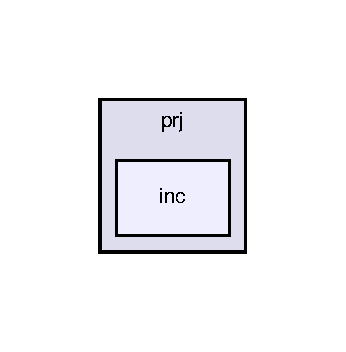
\includegraphics[width=166pt]{dir_c20e5da57ddf016417026fe54ca60b20_dep}
\end{center}
\end{figure}
\subsection*{\-Pliki}
\begin{DoxyCompactItemize}
\item 
plik \hyperlink{algorytm_8hh}{algorytm.\-hh}
\begin{DoxyCompactList}\small\item\em \-Definicja klas wykonujacych operacje na zestawie danych wejsciowych. \end{DoxyCompactList}\item 
plik \hyperlink{operacje_8hh}{operacje.\-hh}
\item 
plik \hyperlink{statystyki_8hh}{statystyki.\-hh}
\begin{DoxyCompactList}\small\item\em plik zawiera dekalracje funkcji odpowiedzialnych za przeprowadznaie statystyk \end{DoxyCompactList}\end{DoxyCompactItemize}

\hypertarget{dir_290162856a453f1bb77275150ef3dd18}{\section{\-Dokumentacja katalogu /home/pwilkosz/pamsi/lab1/prj/}
\label{dir_290162856a453f1bb77275150ef3dd18}\index{\-Dokumentacja katalogu /home/pwilkosz/pamsi/lab1/prj/@{\-Dokumentacja katalogu /home/pwilkosz/pamsi/lab1/prj/}}
}
\-Directory dependency graph for /home/pwilkosz/pamsi/lab1/prj/\-:
\nopagebreak
\begin{figure}[H]
\begin{center}
\leavevmode
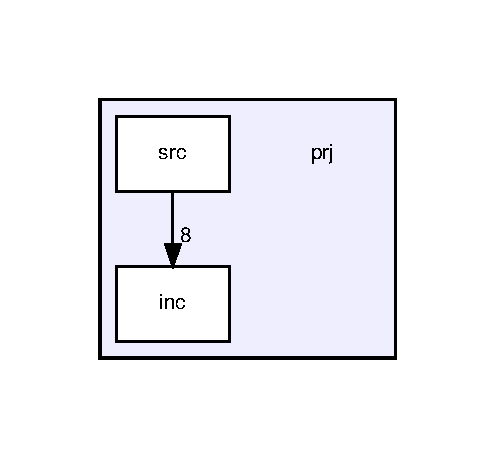
\includegraphics[width=238pt]{dir_290162856a453f1bb77275150ef3dd18_dep}
\end{center}
\end{figure}
\subsection*{\-Katalogi}
\begin{DoxyCompactItemize}
\item 
katalog \hyperlink{dir_c20e5da57ddf016417026fe54ca60b20}{inc}
\item 
katalog \hyperlink{dir_d6fa5e206d9d4500e700eacdb543ed10}{src}
\end{DoxyCompactItemize}

\hypertarget{dir_d6fa5e206d9d4500e700eacdb543ed10}{\section{\-Dokumentacja katalogu /home/pwilkosz/pamsi/lab1/prj/src/}
\label{dir_d6fa5e206d9d4500e700eacdb543ed10}\index{\-Dokumentacja katalogu /home/pwilkosz/pamsi/lab1/prj/src/@{\-Dokumentacja katalogu /home/pwilkosz/pamsi/lab1/prj/src/}}
}
\-Directory dependency graph for /home/pwilkosz/pamsi/lab1/prj/src/\-:
\nopagebreak
\begin{figure}[H]
\begin{center}
\leavevmode
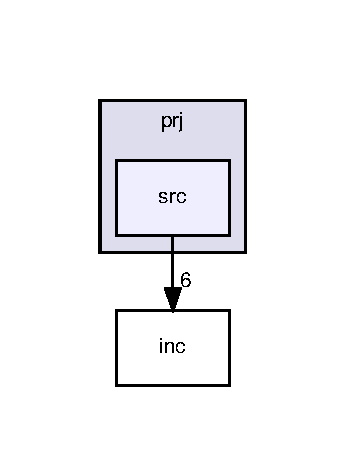
\includegraphics[width=166pt]{dir_d6fa5e206d9d4500e700eacdb543ed10_dep}
\end{center}
\end{figure}
\subsection*{\-Pliki}
\begin{DoxyCompactItemize}
\item 
plik \hyperlink{algorytm_8cpp}{algorytm.\-cpp}
\begin{DoxyCompactList}\small\item\em plik zawiera definicje metod klas zdefiniowanych w pliku \hyperlink{algorytm_8hh}{algorytm.\-hh} \end{DoxyCompactList}\item 
plik \hyperlink{main_8cpp}{main.\-cpp}
\begin{DoxyCompactList}\small\item\em plik glowny \end{DoxyCompactList}\item 
plik \hyperlink{operacje_8cpp}{operacje.\-cpp}
\item 
plik \hyperlink{statystyki_8cpp}{statystyki.\-cpp}
\end{DoxyCompactItemize}

\chapter{\-Dokumentacja klas}
\hypertarget{classalgorytm}{\section{\-Dokumentacja klasy algorytm}
\label{classalgorytm}\index{algorytm@{algorytm}}
}


\-Definicja klasy algorytm \-Jest to klasa bazowa, ktora ma za zadanie wczytac, przetworzyc i porownac plik z plikiem wzorcowym.  




{\ttfamily \#include $<$algorytm.\-hh$>$}



\-Diagram dziedziczenia dla algorytm
\nopagebreak
\begin{figure}[H]
\begin{center}
\leavevmode
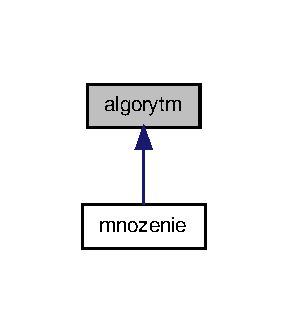
\includegraphics[width=138pt]{classalgorytm__inherit__graph}
\end{center}
\end{figure}
\subsection*{\-Metody publiczne}
\begin{DoxyCompactItemize}
\item 
\hyperlink{classalgorytm_a138ed27849535b192fec3d2e9f6a644f}{algorytm} (const char $\ast$plik1, const char $\ast$plik2)
\begin{DoxyCompactList}\small\item\em konstruktor kopiujacy -\/ przekazuje informacje o nazwach plikow, ktore zapisywane sa do pol klasy \end{DoxyCompactList}\item 
virtual void \hyperlink{classalgorytm_a85ba543fad39e8987bbda4ee698b5fec}{wykonaj} ()
\begin{DoxyCompactList}\small\item\em funkcja dokonuje operacji na pliku wejsciowym \end{DoxyCompactList}\item 
bool \hyperlink{classalgorytm_a167adca6239e12cb5d362fd7c905dde0}{porownaj} ()
\begin{DoxyCompactList}\small\item\em porownuje przetworzony plik z plikiem wzorcowym \end{DoxyCompactList}\item 
int \hyperlink{classalgorytm_acbd9260a0b2055acee485f737b960992}{ile\-\_\-danych} ()
\item 
vector$<$ float $>$ \hyperlink{classalgorytm_a244d9cbf20639faf0b60ae6cdae3c657}{jaki\-\_\-czas} ()
\end{DoxyCompactItemize}
\subsection*{\-Atrybuty publiczne}
\begin{DoxyCompactItemize}
\item 
vector$<$ float $>$ \hyperlink{classalgorytm_aac9e2179e0e956dbe0dc1239ebadb2e4}{czas}
\begin{DoxyCompactList}\small\item\em zawiera wyniki dzialania algorytmu \end{DoxyCompactList}\end{DoxyCompactItemize}
\subsection*{\-Atrybuty chronione}
\begin{DoxyCompactItemize}
\item 
int \hyperlink{classalgorytm_a2778c37f0ec06a30b7d494501c40e91a}{n}
\begin{DoxyCompactList}\small\item\em zawiera informacje o ilosci liczb w pliku \end{DoxyCompactList}\item 
const char $\ast$ \hyperlink{classalgorytm_ab911ca0437df967d0240651855e5a2a3}{plik\-We}
\begin{DoxyCompactList}\small\item\em zawiera nazwe pliku wejsciowego \end{DoxyCompactList}\item 
const char $\ast$ \hyperlink{classalgorytm_a19c2be15efb3e5e34bf177d50b746d93}{plik\-Wz}
\begin{DoxyCompactList}\small\item\em zawiera nazwe pliku wzorcowego \end{DoxyCompactList}\end{DoxyCompactItemize}


\subsection{\-Opis szczegółowy}
\-Definicja klasy algorytm \-Jest to klasa bazowa, ktora ma za zadanie wczytac, przetworzyc i porownac plik z plikiem wzorcowym. 

\-Definicja w linii 32 pliku algorytm.\-hh.



\subsection{\-Dokumentacja konstruktora i destruktora}
\hypertarget{classalgorytm_a138ed27849535b192fec3d2e9f6a644f}{\index{algorytm@{algorytm}!algorytm@{algorytm}}
\index{algorytm@{algorytm}!algorytm@{algorytm}}
\subsubsection[{algorytm}]{\setlength{\rightskip}{0pt plus 5cm}{\bf algorytm\-::algorytm} (
\begin{DoxyParamCaption}
\item[{const char $\ast$}]{plik1, }
\item[{const char $\ast$}]{plik2}
\end{DoxyParamCaption}
)\hspace{0.3cm}{\ttfamily  \mbox{[}inline\mbox{]}}}}\label{classalgorytm_a138ed27849535b192fec3d2e9f6a644f}


konstruktor kopiujacy -\/ przekazuje informacje o nazwach plikow, ktore zapisywane sa do pol klasy 


\begin{DoxyParams}{\-Parametry}
{\em plik1} & -\/ plik wejsciowy \\
\hline
{\em plik2} & -\/ plik wzorcowy \\
\hline
\end{DoxyParams}


\-Definicja w linii 56 pliku algorytm.\-hh.



\subsection{\-Dokumentacja funkcji składowych}
\hypertarget{classalgorytm_acbd9260a0b2055acee485f737b960992}{\index{algorytm@{algorytm}!ile\-\_\-danych@{ile\-\_\-danych}}
\index{ile\-\_\-danych@{ile\-\_\-danych}!algorytm@{algorytm}}
\subsubsection[{ile\-\_\-danych}]{\setlength{\rightskip}{0pt plus 5cm}int {\bf algorytm\-::ile\-\_\-danych} (
\begin{DoxyParamCaption}
{}
\end{DoxyParamCaption}
)}}\label{classalgorytm_acbd9260a0b2055acee485f737b960992}
\begin{DoxyReturn}{\-Zwraca}
ilosc liczb wejsciowych 
\end{DoxyReturn}


\-Definicja w linii 16 pliku algorytm.\-cpp.

\hypertarget{classalgorytm_a244d9cbf20639faf0b60ae6cdae3c657}{\index{algorytm@{algorytm}!jaki\-\_\-czas@{jaki\-\_\-czas}}
\index{jaki\-\_\-czas@{jaki\-\_\-czas}!algorytm@{algorytm}}
\subsubsection[{jaki\-\_\-czas}]{\setlength{\rightskip}{0pt plus 5cm}vector$<$ float $>$ {\bf algorytm\-::jaki\-\_\-czas} (
\begin{DoxyParamCaption}
{}
\end{DoxyParamCaption}
)}}\label{classalgorytm_a244d9cbf20639faf0b60ae6cdae3c657}


\-Definicja w linii 19 pliku algorytm.\-cpp.

\hypertarget{classalgorytm_a167adca6239e12cb5d362fd7c905dde0}{\index{algorytm@{algorytm}!porownaj@{porownaj}}
\index{porownaj@{porownaj}!algorytm@{algorytm}}
\subsubsection[{porownaj}]{\setlength{\rightskip}{0pt plus 5cm}bool {\bf algorytm\-::porownaj} (
\begin{DoxyParamCaption}
{}
\end{DoxyParamCaption}
)}}\label{classalgorytm_a167adca6239e12cb5d362fd7c905dde0}


porownuje przetworzony plik z plikiem wzorcowym 

\begin{DoxyReturn}{\-Zwraca}
true -\/ gdy pliki zgodne false -\/ w przeciwnym przypadku 
\end{DoxyReturn}


\-Definicja w linii 23 pliku algorytm.\-cpp.



\-Oto graf wywoływań tej funkcji\-:
\nopagebreak
\begin{figure}[H]
\begin{center}
\leavevmode
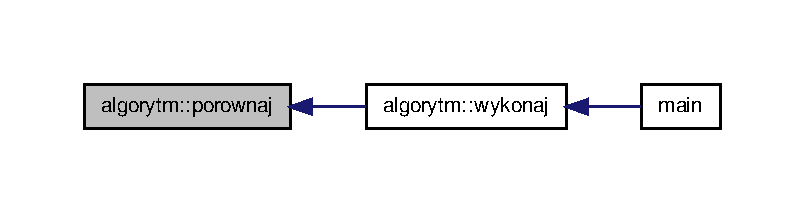
\includegraphics[width=350pt]{classalgorytm_a167adca6239e12cb5d362fd7c905dde0_icgraph}
\end{center}
\end{figure}


\hypertarget{classalgorytm_a85ba543fad39e8987bbda4ee698b5fec}{\index{algorytm@{algorytm}!wykonaj@{wykonaj}}
\index{wykonaj@{wykonaj}!algorytm@{algorytm}}
\subsubsection[{wykonaj}]{\setlength{\rightskip}{0pt plus 5cm}void {\bf algorytm\-::wykonaj} (
\begin{DoxyParamCaption}
{}
\end{DoxyParamCaption}
)\hspace{0.3cm}{\ttfamily  \mbox{[}virtual\mbox{]}}}}\label{classalgorytm_a85ba543fad39e8987bbda4ee698b5fec}


funkcja dokonuje operacji na pliku wejsciowym 



\-Reimplementowana w \hyperlink{classmnozenie_a2c5dc64610bb16af0ef18d142d6af2c0}{mnozenie}.



\-Definicja w linii 7 pliku algorytm.\-cpp.



\subsection{\-Dokumentacja atrybutów składowych}
\hypertarget{classalgorytm_aac9e2179e0e956dbe0dc1239ebadb2e4}{\index{algorytm@{algorytm}!czas@{czas}}
\index{czas@{czas}!algorytm@{algorytm}}
\subsubsection[{czas}]{\setlength{\rightskip}{0pt plus 5cm}vector$<$float$>$ {\bf algorytm\-::czas}}}\label{classalgorytm_aac9e2179e0e956dbe0dc1239ebadb2e4}


zawiera wyniki dzialania algorytmu 



\-Definicja w linii 50 pliku algorytm.\-hh.

\hypertarget{classalgorytm_a2778c37f0ec06a30b7d494501c40e91a}{\index{algorytm@{algorytm}!n@{n}}
\index{n@{n}!algorytm@{algorytm}}
\subsubsection[{n}]{\setlength{\rightskip}{0pt plus 5cm}int {\bf algorytm\-::n}\hspace{0.3cm}{\ttfamily  \mbox{[}protected\mbox{]}}}}\label{classalgorytm_a2778c37f0ec06a30b7d494501c40e91a}


zawiera informacje o ilosci liczb w pliku 



\-Definicja w linii 37 pliku algorytm.\-hh.

\hypertarget{classalgorytm_ab911ca0437df967d0240651855e5a2a3}{\index{algorytm@{algorytm}!plik\-We@{plik\-We}}
\index{plik\-We@{plik\-We}!algorytm@{algorytm}}
\subsubsection[{plik\-We}]{\setlength{\rightskip}{0pt plus 5cm}const char$\ast$ {\bf algorytm\-::plik\-We}\hspace{0.3cm}{\ttfamily  \mbox{[}protected\mbox{]}}}}\label{classalgorytm_ab911ca0437df967d0240651855e5a2a3}


zawiera nazwe pliku wejsciowego 



\-Definicja w linii 41 pliku algorytm.\-hh.

\hypertarget{classalgorytm_a19c2be15efb3e5e34bf177d50b746d93}{\index{algorytm@{algorytm}!plik\-Wz@{plik\-Wz}}
\index{plik\-Wz@{plik\-Wz}!algorytm@{algorytm}}
\subsubsection[{plik\-Wz}]{\setlength{\rightskip}{0pt plus 5cm}const char$\ast$ {\bf algorytm\-::plik\-Wz}\hspace{0.3cm}{\ttfamily  \mbox{[}protected\mbox{]}}}}\label{classalgorytm_a19c2be15efb3e5e34bf177d50b746d93}


zawiera nazwe pliku wzorcowego 



\-Definicja w linii 45 pliku algorytm.\-hh.



\-Dokumentacja dla tej klasy została wygenerowana z plików\-:\begin{DoxyCompactItemize}
\item 
\hyperlink{algorytm_8hh}{algorytm.\-hh}\item 
\hyperlink{algorytm_8cpp}{algorytm.\-cpp}\end{DoxyCompactItemize}

\hypertarget{classmnozenie}{\section{\-Dokumentacja klasy mnozenie}
\label{classmnozenie}\index{mnozenie@{mnozenie}}
}


modeluje algorytm dokonujacy mnozenia kazdego elementu pliku wejsciowego przez 2  




{\ttfamily \#include $<$algorytm.\-hh$>$}



\-Diagram dziedziczenia dla mnozenie\nopagebreak
\begin{figure}[H]
\begin{center}
\leavevmode
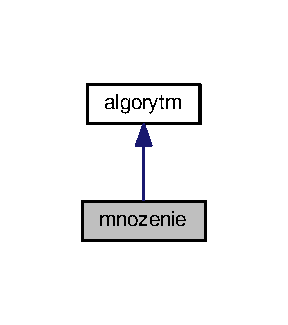
\includegraphics[width=138pt]{classmnozenie__inherit__graph}
\end{center}
\end{figure}


\-Diagram współpracy dla mnozenie\-:\nopagebreak
\begin{figure}[H]
\begin{center}
\leavevmode
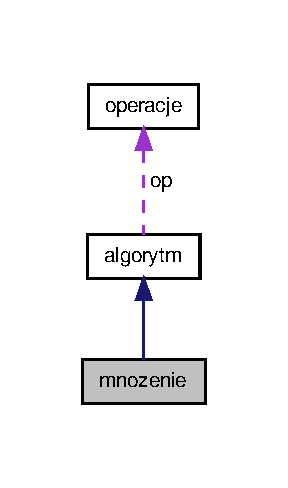
\includegraphics[width=138pt]{classmnozenie__coll__graph}
\end{center}
\end{figure}
\subsection*{\-Metody publiczne}
\begin{DoxyCompactItemize}
\item 
\hyperlink{classmnozenie_a105c483d60c621dc5c1855a04e285e3c}{mnozenie} (ifstream \&plik1, ifstream \&plik2, int \-N, int \-M)
\item 
void \hyperlink{classmnozenie_a5c97c36f9463bdf4eb7e34976a029930}{przelicz} ()
\begin{DoxyCompactList}\small\item\em wykonuje zalozony algorytm mnozenia elementow tablicy przez 2 \end{DoxyCompactList}\end{DoxyCompactItemize}


\subsection{\-Opis szczegółowy}
modeluje algorytm dokonujacy mnozenia kazdego elementu pliku wejsciowego przez 2 

\-Definicja w linii 125 pliku algorytm.\-hh.



\subsection{\-Dokumentacja konstruktora i destruktora}
\hypertarget{classmnozenie_a105c483d60c621dc5c1855a04e285e3c}{\index{mnozenie@{mnozenie}!mnozenie@{mnozenie}}
\index{mnozenie@{mnozenie}!mnozenie@{mnozenie}}
\subsubsection[{mnozenie}]{\setlength{\rightskip}{0pt plus 5cm}{\bf mnozenie\-::mnozenie} (
\begin{DoxyParamCaption}
\item[{ifstream \&}]{plik1, }
\item[{ifstream \&}]{plik2, }
\item[{int}]{\-N, }
\item[{int}]{\-M}
\end{DoxyParamCaption}
)\hspace{0.3cm}{\ttfamily  \mbox{[}inline\mbox{]}}}}\label{classmnozenie_a105c483d60c621dc5c1855a04e285e3c}
/brief konstruktor przekazuje do pol klasy informacje o nazwach pliku wejsciowego i wzorcowego 
\begin{DoxyParams}[1]{\-Parametry}
\mbox{\tt in}  & {\em plik1} & -\/ plik wejsciowy \\
\hline
\mbox{\tt in}  & {\em plik2} & -\/ plik wzorcowy \\
\hline
\mbox{\tt in}  & {\em \-N} & -\/ ilosc danych wejsciowych \\
\hline
\mbox{\tt in}  & {\em \-M} & -\/ ilosc powtorzen \\
\hline
\end{DoxyParams}


\-Definicja w linii 134 pliku algorytm.\-hh.



\subsection{\-Dokumentacja funkcji składowych}
\hypertarget{classmnozenie_a5c97c36f9463bdf4eb7e34976a029930}{\index{mnozenie@{mnozenie}!przelicz@{przelicz}}
\index{przelicz@{przelicz}!mnozenie@{mnozenie}}
\subsubsection[{przelicz}]{\setlength{\rightskip}{0pt plus 5cm}void {\bf mnozenie\-::przelicz} (
\begin{DoxyParamCaption}
{}
\end{DoxyParamCaption}
)\hspace{0.3cm}{\ttfamily  \mbox{[}virtual\mbox{]}}}}\label{classmnozenie_a5c97c36f9463bdf4eb7e34976a029930}


wykonuje zalozony algorytm mnozenia elementow tablicy przez 2 



\-Reimplementowana z \hyperlink{classalgorytm_aeefdd677ca8b9475a15547dcf8dd461f}{algorytm}.



\-Definicja w linii 81 pliku algorytm.\-cpp.



\-Dokumentacja dla tej klasy została wygenerowana z plików\-:\begin{DoxyCompactItemize}
\item 
\hyperlink{algorytm_8hh}{algorytm.\-hh}\item 
\hyperlink{algorytm_8cpp}{algorytm.\-cpp}\end{DoxyCompactItemize}

\hypertarget{classoperacje}{\section{\-Dokumentacja klasy operacje}
\label{classoperacje}\index{operacje@{operacje}}
}


\-Klasa modeluje tablice z danymi i metody sluzace do operacji na niej.  




{\ttfamily \#include $<$operacje.\-hh$>$}

\subsection*{\-Metody publiczne}
\begin{DoxyCompactItemize}
\item 
\hyperlink{classoperacje_a4538e0bfde26291449dc057134b23ad8}{operacje} ()
\begin{DoxyCompactList}\small\item\em konstruktor bezparametryczny \end{DoxyCompactList}\item 
\hyperlink{classoperacje_af109f7f9a4b10334d5e8c215c7f220de}{operacje} (int \-N)
\begin{DoxyCompactList}\small\item\em konstruktor parametryczny -\/ alokuje pamiec w dynamicznej tablicy {\ttfamily tab} \end{DoxyCompactList}\item 
bool \hyperlink{classoperacje_a7393a8b3b394921a084e0c1f4ad517b7}{zamien\-\_\-elementy} (int i, int j)
\begin{DoxyCompactList}\small\item\em \-Metoda zamienia 2 elementy tablicy. \end{DoxyCompactList}\item 
void \hyperlink{classoperacje_a7aa29c588e5a8f93c437150f03a133f1}{quick\-\_\-sort} (int l, int p)
\begin{DoxyCompactList}\small\item\em \-Metoda \-Dokonuje sortownaia szybkiego. \end{DoxyCompactList}\item 
void \hyperlink{classoperacje_a9be241905b909e7aef0151902c6f5b81}{make\-\_\-node} (int rozmiar, int i)
\begin{DoxyCompactList}\small\item\em \-Metoda tworzy wezel drzewa, przypisujac mu 2 synow, ustawiajac ich w odpowiedniej kolejnosci (ojciec ma najwieksza wartosc) \end{DoxyCompactList}\item 
void \hyperlink{classoperacje_ae752685beea6c7ee81d2347a98d40146}{make\-\_\-heap} ()
\begin{DoxyCompactList}\small\item\em \-Metoda tworzy kopiec binarny. \end{DoxyCompactList}\item 
void \hyperlink{classoperacje_aec9d2248eb072f97da794ee4c9b99a5d}{heap\-\_\-sort} ()
\begin{DoxyCompactList}\small\item\em \-Metoda dokonuje sortowania po uprzednim utworzeniu kopca. \end{DoxyCompactList}\item 
void \hyperlink{classoperacje_ad766f1d18595ff6b779485528c65d3f0}{merge} (int poczatek, int srodek, int koniec)
\begin{DoxyCompactList}\small\item\em \-Metoda scala dwie czesci tablicy, jednoczesnie je porzadkujac. \end{DoxyCompactList}\item 
void \hyperlink{classoperacje_ac65f2613b7d32b4f95e59bf2f8fd1aab}{merge\-\_\-sort} (int poczatek, int koniec)
\item 
void \hyperlink{classoperacje_aedc47c87f4f44f8af0cba64a940a5333}{odwroc\-\_\-tablice} ()
\begin{DoxyCompactList}\small\item\em metoda odwraca wszystkie elementy tablicy \end{DoxyCompactList}\item 
void \hyperlink{classoperacje_ad8397efded792c1381bfd0292b3e91b6}{dodaj\-\_\-element} (float e)
\begin{DoxyCompactList}\small\item\em metoda dodaje element do tablicy, alokujac dodatkowa pamiec \end{DoxyCompactList}\item 
void \hyperlink{classoperacje_a933533caa39434db543aca704804625c}{dodaj\-\_\-elementy} (float $\ast$tab2, int rozm)
\begin{DoxyCompactList}\small\item\em metoda dodaje elementy do tablicy \end{DoxyCompactList}\item 
void \hyperlink{classoperacje_a33127b613894949faba7a04f23075bf8}{operator=} (float $\ast$tab1)
\begin{DoxyCompactList}\small\item\em \-Przeciazenie operatora przypisania; przypisuje elementy tablicy {\ttfamily tab1} {\ttfamily do} tablicy bedacej polem klasy. \end{DoxyCompactList}\item 
bool \hyperlink{classoperacje_af69f25c4d1da5a7e46ff21a56143fc62}{operator==} (float $\ast$tab1)
\begin{DoxyCompactList}\small\item\em \-Przeciazenie operatora porownania; metoda porownuje zawartosci dwoch tablic. \end{DoxyCompactList}\item 
float \& \hyperlink{classoperacje_a6aeba674ecf3058e63e12bca9862a7fb}{operator\mbox{[}$\,$\mbox{]}} (int ind)
\end{DoxyCompactItemize}
\subsection*{\-Atrybuty publiczne}
\begin{DoxyCompactItemize}
\item 
int \hyperlink{classoperacje_aec7cc301d8822128d918aa1f9c7e1db2}{n}
\begin{DoxyCompactList}\small\item\em ilosc elementow w tablicy \end{DoxyCompactList}\item 
float $\ast$ \hyperlink{classoperacje_ad23bc418eebc9b493a5494ffd9358dd0}{tab}
\begin{DoxyCompactList}\small\item\em tablica z liczbami \end{DoxyCompactList}\end{DoxyCompactItemize}


\subsection{\-Opis szczegółowy}
\-Klasa modeluje tablice z danymi i metody sluzace do operacji na niej. 

\-Definicja w linii 11 pliku operacje.\-hh.



\subsection{\-Dokumentacja konstruktora i destruktora}
\hypertarget{classoperacje_a4538e0bfde26291449dc057134b23ad8}{\index{operacje@{operacje}!operacje@{operacje}}
\index{operacje@{operacje}!operacje@{operacje}}
\subsubsection[{operacje}]{\setlength{\rightskip}{0pt plus 5cm}{\bf operacje\-::operacje} (
\begin{DoxyParamCaption}
{}
\end{DoxyParamCaption}
)}}\label{classoperacje_a4538e0bfde26291449dc057134b23ad8}


konstruktor bezparametryczny 

\hypertarget{classoperacje_af109f7f9a4b10334d5e8c215c7f220de}{\index{operacje@{operacje}!operacje@{operacje}}
\index{operacje@{operacje}!operacje@{operacje}}
\subsubsection[{operacje}]{\setlength{\rightskip}{0pt plus 5cm}{\bf operacje\-::operacje} (
\begin{DoxyParamCaption}
\item[{int}]{\-N}
\end{DoxyParamCaption}
)\hspace{0.3cm}{\ttfamily  \mbox{[}inline\mbox{]}}}}\label{classoperacje_af109f7f9a4b10334d5e8c215c7f220de}


konstruktor parametryczny -\/ alokuje pamiec w dynamicznej tablicy {\ttfamily tab} 


\begin{DoxyParams}[1]{\-Parametry}
\mbox{\tt in}  & {\em \-N} & -\/ ilosc elementow w tablicy; parametr przypisywany do pola {\ttfamily n} w klasie, oraz alokuje pamiec o takim wlasnie rozmiarze \\
\hline
\end{DoxyParams}


\-Definicja w linii 28 pliku operacje.\-hh.



\subsection{\-Dokumentacja funkcji składowych}
\hypertarget{classoperacje_ad8397efded792c1381bfd0292b3e91b6}{\index{operacje@{operacje}!dodaj\-\_\-element@{dodaj\-\_\-element}}
\index{dodaj\-\_\-element@{dodaj\-\_\-element}!operacje@{operacje}}
\subsubsection[{dodaj\-\_\-element}]{\setlength{\rightskip}{0pt plus 5cm}void {\bf operacje\-::dodaj\-\_\-element} (
\begin{DoxyParamCaption}
\item[{float}]{e}
\end{DoxyParamCaption}
)}}\label{classoperacje_ad8397efded792c1381bfd0292b3e91b6}


metoda dodaje element do tablicy, alokujac dodatkowa pamiec 


\begin{DoxyParams}[1]{\-Parametry}
\mbox{\tt in}  & {\em e} & -\/ element, ktory nalezy dolaczyc do tablicy \\
\hline
\end{DoxyParams}


\-Definicja w linii 27 pliku operacje.\-cpp.

\hypertarget{classoperacje_a933533caa39434db543aca704804625c}{\index{operacje@{operacje}!dodaj\-\_\-elementy@{dodaj\-\_\-elementy}}
\index{dodaj\-\_\-elementy@{dodaj\-\_\-elementy}!operacje@{operacje}}
\subsubsection[{dodaj\-\_\-elementy}]{\setlength{\rightskip}{0pt plus 5cm}void {\bf operacje\-::dodaj\-\_\-elementy} (
\begin{DoxyParamCaption}
\item[{float $\ast$}]{tab2, }
\item[{int}]{rozm}
\end{DoxyParamCaption}
)}}\label{classoperacje_a933533caa39434db543aca704804625c}


metoda dodaje elementy do tablicy 


\begin{DoxyParams}[1]{\-Parametry}
\mbox{\tt in}  & {\em tab2} & -\/ tablica, ktora nalezy dolaczyc \\
\hline
\mbox{\tt in}  & {\em rozm} & -\/ rozmiar tablicy tab2 \\
\hline
\end{DoxyParams}


\-Definicja w linii 46 pliku operacje.\-cpp.

\hypertarget{classoperacje_aec9d2248eb072f97da794ee4c9b99a5d}{\index{operacje@{operacje}!heap\-\_\-sort@{heap\-\_\-sort}}
\index{heap\-\_\-sort@{heap\-\_\-sort}!operacje@{operacje}}
\subsubsection[{heap\-\_\-sort}]{\setlength{\rightskip}{0pt plus 5cm}void {\bf operacje\-::heap\-\_\-sort} (
\begin{DoxyParamCaption}
{}
\end{DoxyParamCaption}
)}}\label{classoperacje_aec9d2248eb072f97da794ee4c9b99a5d}


\-Metoda dokonuje sortowania po uprzednim utworzeniu kopca. 



\-Definicja w linii 116 pliku operacje.\-cpp.



\-Oto graf wywołań dla tej funkcji\-:\nopagebreak
\begin{figure}[H]
\begin{center}
\leavevmode
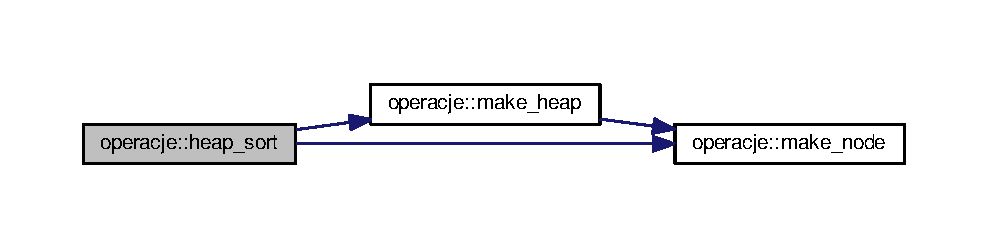
\includegraphics[width=350pt]{classoperacje_aec9d2248eb072f97da794ee4c9b99a5d_cgraph}
\end{center}
\end{figure}




\-Oto graf wywoływań tej funkcji\-:\nopagebreak
\begin{figure}[H]
\begin{center}
\leavevmode
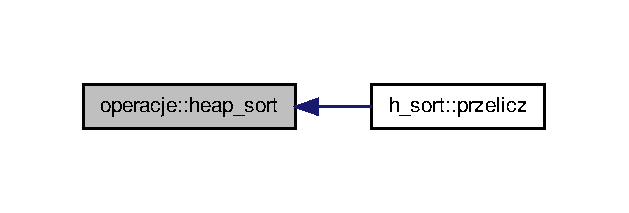
\includegraphics[width=302pt]{classoperacje_aec9d2248eb072f97da794ee4c9b99a5d_icgraph}
\end{center}
\end{figure}


\hypertarget{classoperacje_ae752685beea6c7ee81d2347a98d40146}{\index{operacje@{operacje}!make\-\_\-heap@{make\-\_\-heap}}
\index{make\-\_\-heap@{make\-\_\-heap}!operacje@{operacje}}
\subsubsection[{make\-\_\-heap}]{\setlength{\rightskip}{0pt plus 5cm}void {\bf operacje\-::make\-\_\-heap} (
\begin{DoxyParamCaption}
{}
\end{DoxyParamCaption}
)}}\label{classoperacje_ae752685beea6c7ee81d2347a98d40146}


\-Metoda tworzy kopiec binarny. 



\-Definicja w linii 110 pliku operacje.\-cpp.



\-Oto graf wywołań dla tej funkcji\-:\nopagebreak
\begin{figure}[H]
\begin{center}
\leavevmode
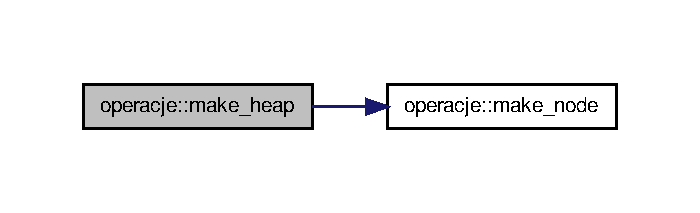
\includegraphics[width=336pt]{classoperacje_ae752685beea6c7ee81d2347a98d40146_cgraph}
\end{center}
\end{figure}




\-Oto graf wywoływań tej funkcji\-:\nopagebreak
\begin{figure}[H]
\begin{center}
\leavevmode
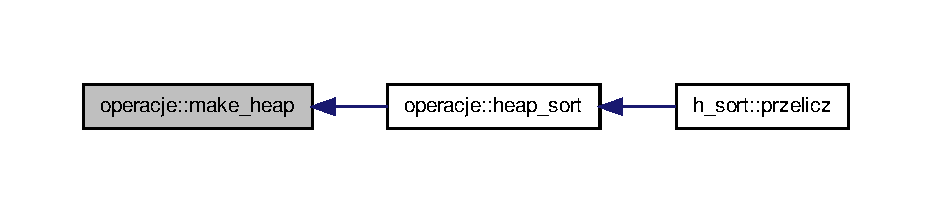
\includegraphics[width=350pt]{classoperacje_ae752685beea6c7ee81d2347a98d40146_icgraph}
\end{center}
\end{figure}


\hypertarget{classoperacje_a9be241905b909e7aef0151902c6f5b81}{\index{operacje@{operacje}!make\-\_\-node@{make\-\_\-node}}
\index{make\-\_\-node@{make\-\_\-node}!operacje@{operacje}}
\subsubsection[{make\-\_\-node}]{\setlength{\rightskip}{0pt plus 5cm}void {\bf operacje\-::make\-\_\-node} (
\begin{DoxyParamCaption}
\item[{int}]{rozmiar, }
\item[{int}]{i}
\end{DoxyParamCaption}
)}}\label{classoperacje_a9be241905b909e7aef0151902c6f5b81}


\-Metoda tworzy wezel drzewa, przypisujac mu 2 synow, ustawiajac ich w odpowiedniej kolejnosci (ojciec ma najwieksza wartosc) 


\begin{DoxyParams}[1]{\-Parametry}
\mbox{\tt in}  & {\em rozmiar} & -\/ rozmiar tablicy \\
\hline
\mbox{\tt in}  & {\em i} & -\/ indeks elementu, do ktorego przypisujemy synow \\
\hline
\end{DoxyParams}


\-Definicja w linii 95 pliku operacje.\-cpp.



\-Oto graf wywoływań tej funkcji\-:\nopagebreak
\begin{figure}[H]
\begin{center}
\leavevmode
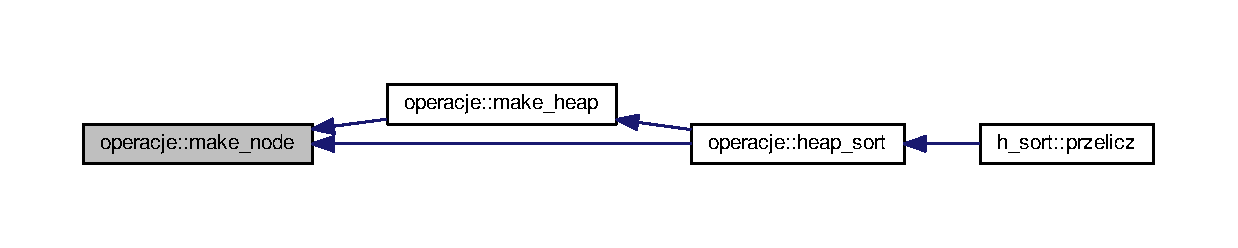
\includegraphics[width=350pt]{classoperacje_a9be241905b909e7aef0151902c6f5b81_icgraph}
\end{center}
\end{figure}


\hypertarget{classoperacje_ad766f1d18595ff6b779485528c65d3f0}{\index{operacje@{operacje}!merge@{merge}}
\index{merge@{merge}!operacje@{operacje}}
\subsubsection[{merge}]{\setlength{\rightskip}{0pt plus 5cm}void {\bf operacje\-::merge} (
\begin{DoxyParamCaption}
\item[{int}]{poczatek, }
\item[{int}]{srodek, }
\item[{int}]{koniec}
\end{DoxyParamCaption}
)}}\label{classoperacje_ad766f1d18595ff6b779485528c65d3f0}


\-Metoda scala dwie czesci tablicy, jednoczesnie je porzadkujac. 


\begin{DoxyParams}[1]{\-Parametry}
\mbox{\tt in}  & {\em poczatek} & -\/ pierwszy indeks tablicy \\
\hline
\mbox{\tt in}  & {\em srodek} & -\/ srodkowy indeks tablicy \\
\hline
\mbox{\tt in}  & {\em koniec} & -\/ ostatni indeks tablicy \\
\hline
\end{DoxyParams}


\-Definicja w linii 130 pliku operacje.\-cpp.



\-Oto graf wywoływań tej funkcji\-:\nopagebreak
\begin{figure}[H]
\begin{center}
\leavevmode
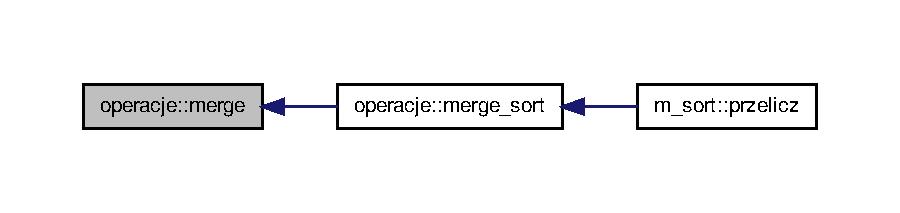
\includegraphics[width=350pt]{classoperacje_ad766f1d18595ff6b779485528c65d3f0_icgraph}
\end{center}
\end{figure}


\hypertarget{classoperacje_ac65f2613b7d32b4f95e59bf2f8fd1aab}{\index{operacje@{operacje}!merge\-\_\-sort@{merge\-\_\-sort}}
\index{merge\-\_\-sort@{merge\-\_\-sort}!operacje@{operacje}}
\subsubsection[{merge\-\_\-sort}]{\setlength{\rightskip}{0pt plus 5cm}void {\bf operacje\-::merge\-\_\-sort} (
\begin{DoxyParamCaption}
\item[{int}]{poczatek, }
\item[{int}]{koniec}
\end{DoxyParamCaption}
)}}\label{classoperacje_ac65f2613b7d32b4f95e59bf2f8fd1aab}
$\backslash$ brief \-Metoda dokonuje sortowania poprzez rekurencyjne wywolanie dla obu polow tablic, nastepnie metoda dokonuje scalenia danych 
\begin{DoxyParams}[1]{\-Parametry}
\mbox{\tt in}  & {\em poczatek} & -\/ pierwszy indeks tablicy \\
\hline
\mbox{\tt in}  & {\em koniec} & -\/ ostatni indeks tablicy \\
\hline
\end{DoxyParams}


\-Definicja w linii 166 pliku operacje.\-cpp.



\-Oto graf wywołań dla tej funkcji\-:\nopagebreak
\begin{figure}[H]
\begin{center}
\leavevmode
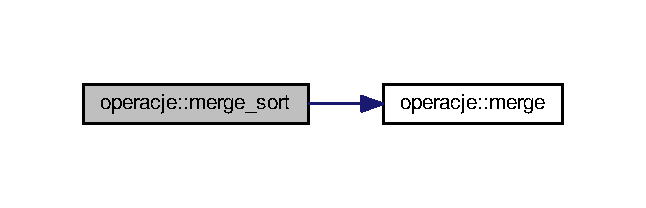
\includegraphics[width=310pt]{classoperacje_ac65f2613b7d32b4f95e59bf2f8fd1aab_cgraph}
\end{center}
\end{figure}




\-Oto graf wywoływań tej funkcji\-:\nopagebreak
\begin{figure}[H]
\begin{center}
\leavevmode
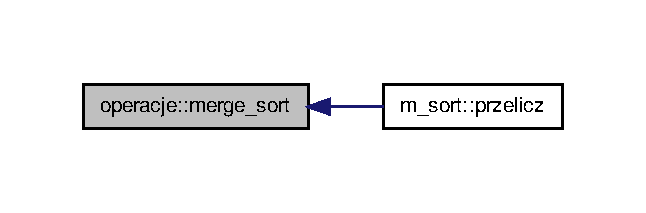
\includegraphics[width=310pt]{classoperacje_ac65f2613b7d32b4f95e59bf2f8fd1aab_icgraph}
\end{center}
\end{figure}


\hypertarget{classoperacje_aedc47c87f4f44f8af0cba64a940a5333}{\index{operacje@{operacje}!odwroc\-\_\-tablice@{odwroc\-\_\-tablice}}
\index{odwroc\-\_\-tablice@{odwroc\-\_\-tablice}!operacje@{operacje}}
\subsubsection[{odwroc\-\_\-tablice}]{\setlength{\rightskip}{0pt plus 5cm}void {\bf operacje\-::odwroc\-\_\-tablice} (
\begin{DoxyParamCaption}
{}
\end{DoxyParamCaption}
)}}\label{classoperacje_aedc47c87f4f44f8af0cba64a940a5333}


metoda odwraca wszystkie elementy tablicy 



\-Definicja w linii 12 pliku operacje.\-cpp.

\hypertarget{classoperacje_a33127b613894949faba7a04f23075bf8}{\index{operacje@{operacje}!operator=@{operator=}}
\index{operator=@{operator=}!operacje@{operacje}}
\subsubsection[{operator=}]{\setlength{\rightskip}{0pt plus 5cm}void operacje\-::operator= (
\begin{DoxyParamCaption}
\item[{float $\ast$}]{tab1}
\end{DoxyParamCaption}
)}}\label{classoperacje_a33127b613894949faba7a04f23075bf8}


\-Przeciazenie operatora przypisania; przypisuje elementy tablicy {\ttfamily tab1} {\ttfamily do} tablicy bedacej polem klasy. 


\begin{DoxyParams}[1]{\-Parametry}
\mbox{\tt in}  & {\em tab1} & -\/ tablica, ktorej zawartosc przypisujemy \\
\hline
\end{DoxyParams}


\-Definicja w linii 63 pliku operacje.\-cpp.

\hypertarget{classoperacje_af69f25c4d1da5a7e46ff21a56143fc62}{\index{operacje@{operacje}!operator==@{operator==}}
\index{operator==@{operator==}!operacje@{operacje}}
\subsubsection[{operator==}]{\setlength{\rightskip}{0pt plus 5cm}bool operacje\-::operator== (
\begin{DoxyParamCaption}
\item[{float $\ast$}]{tab1}
\end{DoxyParamCaption}
)}}\label{classoperacje_af69f25c4d1da5a7e46ff21a56143fc62}


\-Przeciazenie operatora porownania; metoda porownuje zawartosci dwoch tablic. 


\begin{DoxyParams}[1]{\-Parametry}
\mbox{\tt in}  & {\em tab1} & -\/ tablica, ktorej wartosci porownujemy \\
\hline
\end{DoxyParams}
\begin{DoxyReturn}{\-Zwraca}
true -\/ gdy zawartsoc tablic jest identyczna false -\/ w przeciwnym przypadku 
\end{DoxyReturn}


\-Definicja w linii 69 pliku operacje.\-cpp.

\hypertarget{classoperacje_a6aeba674ecf3058e63e12bca9862a7fb}{\index{operacje@{operacje}!operator\mbox{[}$\,$\mbox{]}@{operator[]}}
\index{operator\mbox{[}$\,$\mbox{]}@{operator[]}!operacje@{operacje}}
\subsubsection[{operator[]}]{\setlength{\rightskip}{0pt plus 5cm}float\& operacje\-::operator\mbox{[}$\,$\mbox{]} (
\begin{DoxyParamCaption}
\item[{int}]{ind}
\end{DoxyParamCaption}
)\hspace{0.3cm}{\ttfamily  \mbox{[}inline\mbox{]}}}}\label{classoperacje_a6aeba674ecf3058e63e12bca9862a7fb}


\-Definicja w linii 88 pliku operacje.\-hh.

\hypertarget{classoperacje_a7aa29c588e5a8f93c437150f03a133f1}{\index{operacje@{operacje}!quick\-\_\-sort@{quick\-\_\-sort}}
\index{quick\-\_\-sort@{quick\-\_\-sort}!operacje@{operacje}}
\subsubsection[{quick\-\_\-sort}]{\setlength{\rightskip}{0pt plus 5cm}void {\bf operacje\-::quick\-\_\-sort} (
\begin{DoxyParamCaption}
\item[{int}]{l, }
\item[{int}]{p}
\end{DoxyParamCaption}
)}}\label{classoperacje_a7aa29c588e5a8f93c437150f03a133f1}


\-Metoda \-Dokonuje sortownaia szybkiego. 


\begin{DoxyParams}[1]{\-Parametry}
\mbox{\tt in}  & {\em l} & -\/ pierwszy indeks tablicy \\
\hline
\mbox{\tt in}  & {\em p} & -\/ ostatni indeks tablicy \\
\hline
\end{DoxyParams}


\-Definicja w linii 77 pliku operacje.\-cpp.



\-Oto graf wywołań dla tej funkcji\-:\nopagebreak
\begin{figure}[H]
\begin{center}
\leavevmode
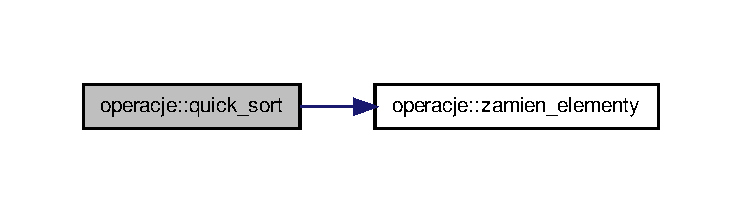
\includegraphics[width=350pt]{classoperacje_a7aa29c588e5a8f93c437150f03a133f1_cgraph}
\end{center}
\end{figure}




\-Oto graf wywoływań tej funkcji\-:\nopagebreak
\begin{figure}[H]
\begin{center}
\leavevmode
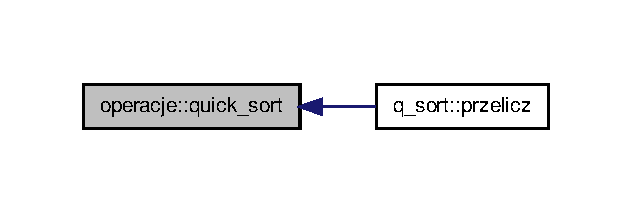
\includegraphics[width=304pt]{classoperacje_a7aa29c588e5a8f93c437150f03a133f1_icgraph}
\end{center}
\end{figure}


\hypertarget{classoperacje_a7393a8b3b394921a084e0c1f4ad517b7}{\index{operacje@{operacje}!zamien\-\_\-elementy@{zamien\-\_\-elementy}}
\index{zamien\-\_\-elementy@{zamien\-\_\-elementy}!operacje@{operacje}}
\subsubsection[{zamien\-\_\-elementy}]{\setlength{\rightskip}{0pt plus 5cm}bool {\bf operacje\-::zamien\-\_\-elementy} (
\begin{DoxyParamCaption}
\item[{int}]{i, }
\item[{int}]{j}
\end{DoxyParamCaption}
)}}\label{classoperacje_a7393a8b3b394921a084e0c1f4ad517b7}


\-Metoda zamienia 2 elementy tablicy. 


\begin{DoxyParams}[1]{\-Parametry}
\mbox{\tt in}  & {\em i} & -\/ element tablicy \\
\hline
\mbox{\tt in}  & {\em j} & -\/ element tablicy \\
\hline
\end{DoxyParams}
\begin{DoxyReturn}{\-Zwraca}
true -\/ gdy elementy nie wykraczaja poza zakres tablicy false -\/ w przeciwnym przypadku 
\end{DoxyReturn}


\-Definicja w linii 3 pliku operacje.\-cpp.



\-Oto graf wywoływań tej funkcji\-:\nopagebreak
\begin{figure}[H]
\begin{center}
\leavevmode
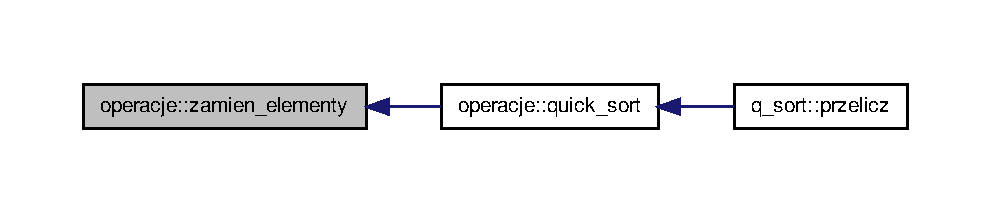
\includegraphics[width=350pt]{classoperacje_a7393a8b3b394921a084e0c1f4ad517b7_icgraph}
\end{center}
\end{figure}




\subsection{\-Dokumentacja atrybutów składowych}
\hypertarget{classoperacje_aec7cc301d8822128d918aa1f9c7e1db2}{\index{operacje@{operacje}!n@{n}}
\index{n@{n}!operacje@{operacje}}
\subsubsection[{n}]{\setlength{\rightskip}{0pt plus 5cm}int {\bf operacje\-::n}}}\label{classoperacje_aec7cc301d8822128d918aa1f9c7e1db2}


ilosc elementow w tablicy 



\-Definicja w linii 16 pliku operacje.\-hh.

\hypertarget{classoperacje_ad23bc418eebc9b493a5494ffd9358dd0}{\index{operacje@{operacje}!tab@{tab}}
\index{tab@{tab}!operacje@{operacje}}
\subsubsection[{tab}]{\setlength{\rightskip}{0pt plus 5cm}float$\ast$ {\bf operacje\-::tab}}}\label{classoperacje_ad23bc418eebc9b493a5494ffd9358dd0}


tablica z liczbami 



\-Definicja w linii 19 pliku operacje.\-hh.



\-Dokumentacja dla tej klasy została wygenerowana z plików\-:\begin{DoxyCompactItemize}
\item 
\hyperlink{operacje_8hh}{operacje.\-hh}\item 
\hyperlink{operacje_8cpp}{operacje.\-cpp}\end{DoxyCompactItemize}

\chapter{\-Dokumentacja plików}
\hypertarget{algorytm_8cpp}{\section{\-Dokumentacja pliku algorytm.\-cpp}
\label{algorytm_8cpp}\index{algorytm.\-cpp@{algorytm.\-cpp}}
}


plik zawiera definicje metod klas zdefiniowanych w pliku \hyperlink{algorytm_8hh}{algorytm.\-hh}  


{\ttfamily \#include \char`\"{}algorytm.\-hh\char`\"{}}\*
\-Wykres zależności załączania dla algorytm.\-cpp\-:
\nopagebreak
\begin{figure}[H]
\begin{center}
\leavevmode
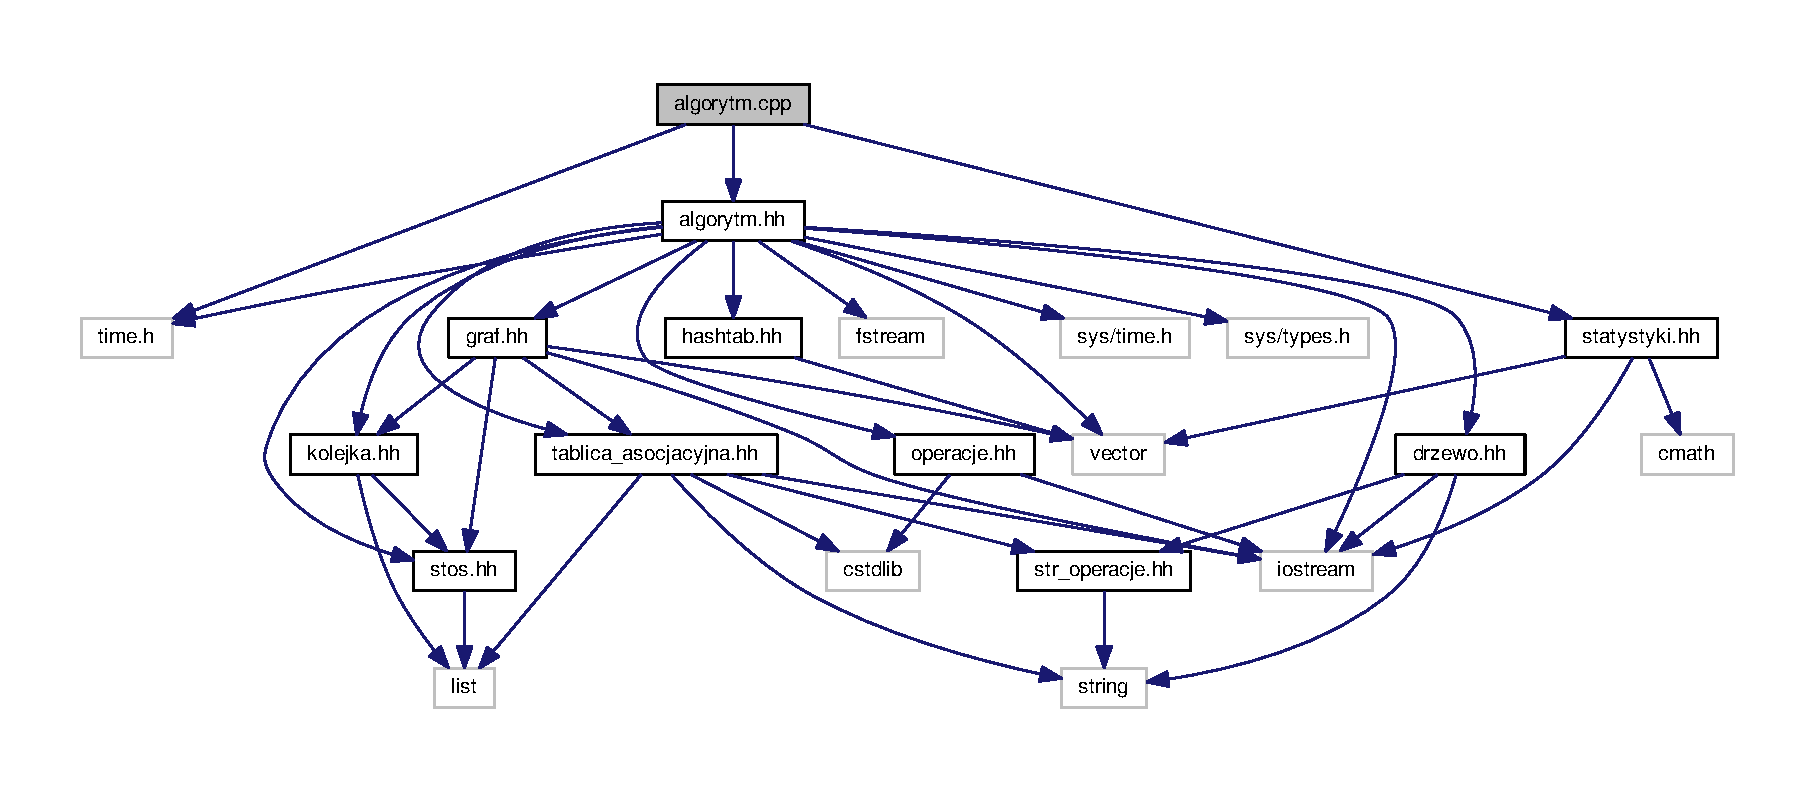
\includegraphics[width=350pt]{algorytm_8cpp__incl}
\end{center}
\end{figure}


\subsection{\-Opis szczegółowy}
plik zawiera definicje metod klas zdefiniowanych w pliku \hyperlink{algorytm_8hh}{algorytm.\-hh} 

\-Definicja w pliku \hyperlink{algorytm_8cpp_source}{algorytm.\-cpp}.


\hypertarget{algorytm_8hh}{\section{\-Dokumentacja pliku algorytm.\-hh}
\label{algorytm_8hh}\index{algorytm.\-hh@{algorytm.\-hh}}
}


\-Definicja klas wykonujacych operacje na zestawie danych wejsciowych.  


{\ttfamily \#include $<$iostream$>$}\*
{\ttfamily \#include $<$fstream$>$}\*
{\ttfamily \#include $<$vector$>$}\*
{\ttfamily \#include $<$ctime$>$}\*
{\ttfamily \#include $<$sys/time.\-h$>$}\*
{\ttfamily \#include $<$sys/types.\-h$>$}\*
\-Wykres zależności załączania dla algorytm.\-hh\-:
\nopagebreak
\begin{figure}[H]
\begin{center}
\leavevmode
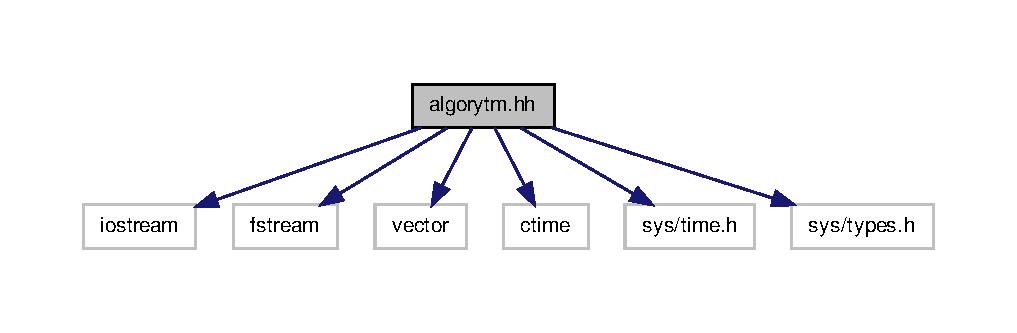
\includegraphics[width=350pt]{algorytm_8hh__incl}
\end{center}
\end{figure}
\-Ten wykres pokazuje, które pliki bezpośrednio lub pośrednio załączają ten plik\-:
\nopagebreak
\begin{figure}[H]
\begin{center}
\leavevmode
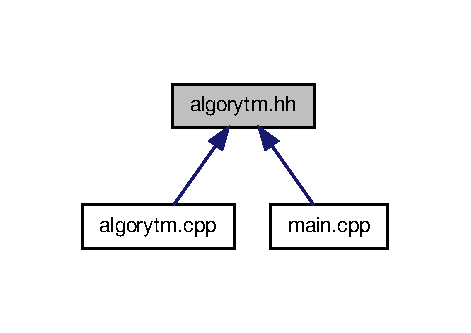
\includegraphics[width=226pt]{algorytm_8hh__dep__incl}
\end{center}
\end{figure}
\subsection*{\-Komponenty}
\begin{DoxyCompactItemize}
\item 
class \hyperlink{classalgorytm}{algorytm}
\begin{DoxyCompactList}\small\item\em \-Definicja klasy algorytm \-Jest to klasa bazowa, ktora ma za zadanie wczytac, przetworzyc i porownac plik z plikiem wzorcowym. \end{DoxyCompactList}\item 
class \hyperlink{classmnozenie}{mnozenie}
\begin{DoxyCompactList}\small\item\em modeluje algorytm dokonujacy mnozenia kazdego elementu pliku wejsciowego przez 2 \end{DoxyCompactList}\end{DoxyCompactItemize}


\subsection{\-Opis szczegółowy}
\-Definicja klas wykonujacych operacje na zestawie danych wejsciowych. 

\-Definicja w pliku \hyperlink{algorytm_8hh_source}{algorytm.\-hh}.


\hypertarget{main_8cpp}{\section{Dokumentacja pliku main.\-cpp}
\label{main_8cpp}\index{main.\-cpp@{main.\-cpp}}
}


plik glowny  


{\ttfamily \#include $<$iostream$>$}\\*
{\ttfamily \#include \char`\"{}algorytm.\-hh\char`\"{}}\\*
{\ttfamily \#include \char`\"{}statystyki.\-hh\char`\"{}}\\*
{\ttfamily \#include \char`\"{}operacje.\-hh\char`\"{}}\\*
{\ttfamily \#include \char`\"{}stos.\-hh\char`\"{}}\\*
{\ttfamily \#include \char`\"{}tablica\-\_\-asocjacyjna.\-hh\char`\"{}}\\*
{\ttfamily \#include \char`\"{}drzewo.\-hh\char`\"{}}\\*
{\ttfamily \#include \char`\"{}hashtab.\-hh\char`\"{}}\\*
{\ttfamily \#include \char`\"{}graf.\-hh\char`\"{}}\\*
{\ttfamily \#include $<$cstdlib$>$}\\*
{\ttfamily \#include $<$string$>$}\\*
Wykres zależności załączania dla main.\-cpp\-:\nopagebreak
\begin{figure}[H]
\begin{center}
\leavevmode
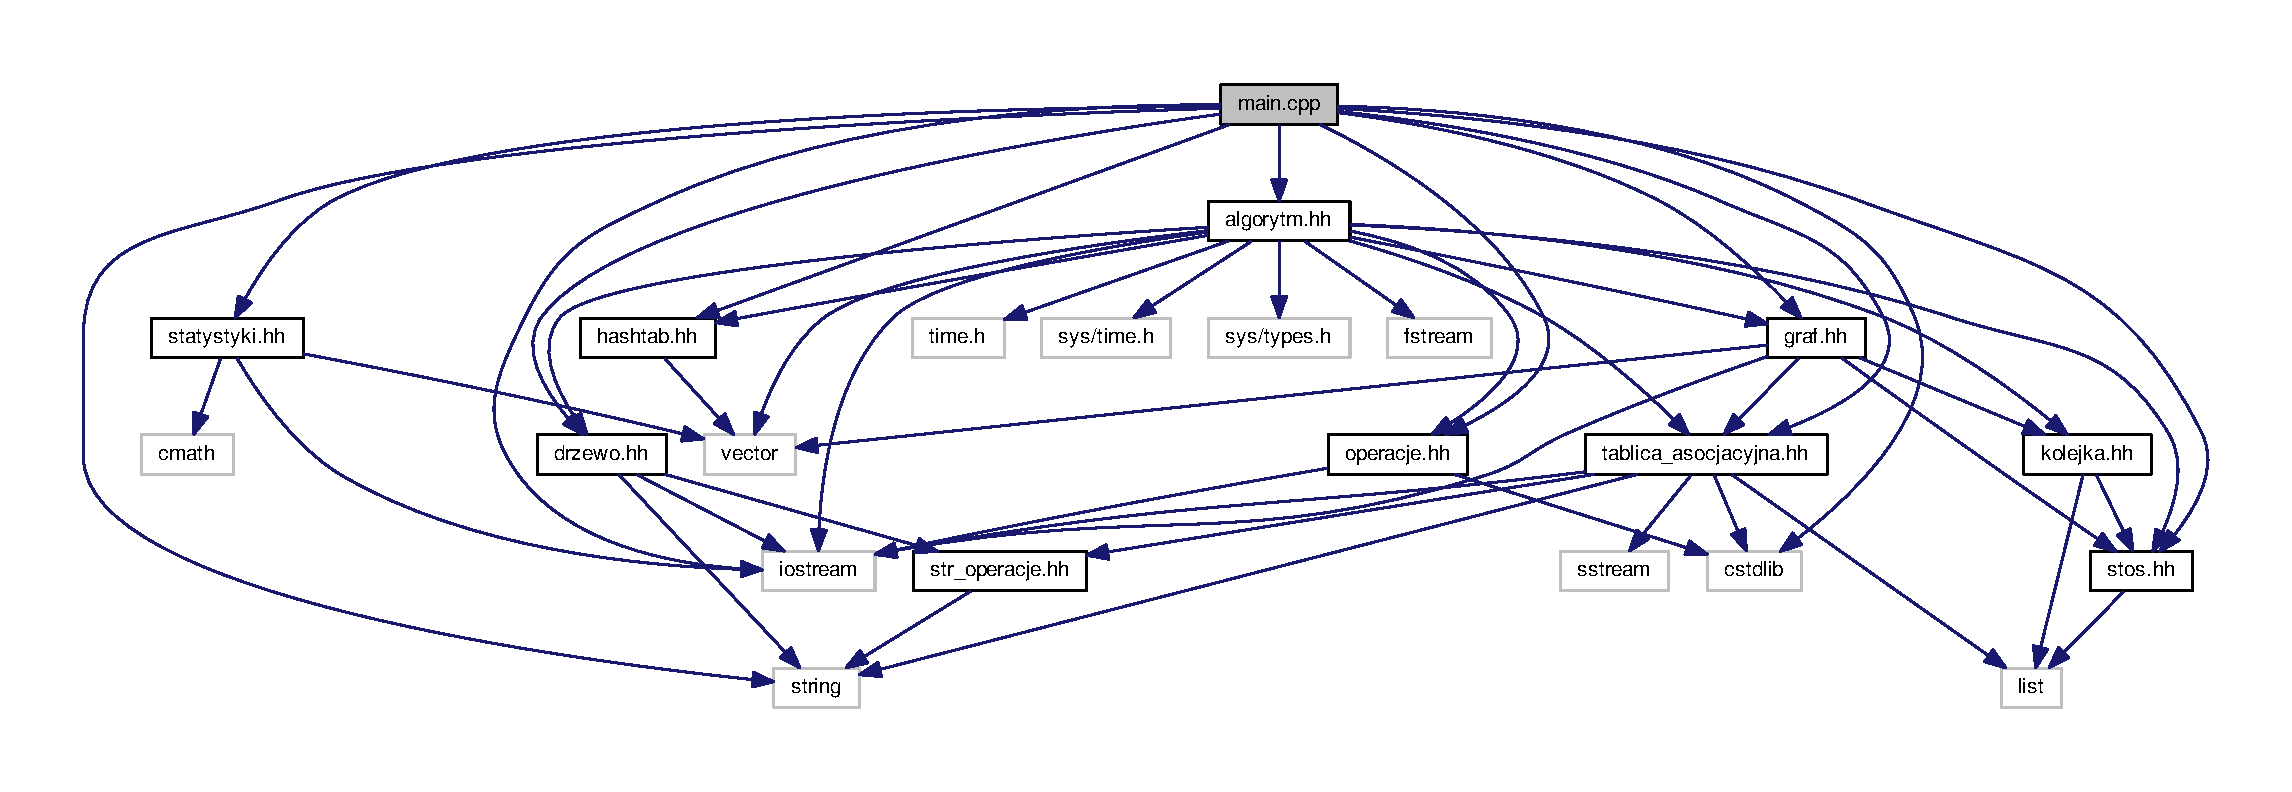
\includegraphics[width=350pt]{main_8cpp__incl}
\end{center}
\end{figure}
\subsection*{Funkcje}
\begin{DoxyCompactItemize}
\item 
int \hyperlink{main_8cpp_ae66f6b31b5ad750f1fe042a706a4e3d4}{main} ()
\end{DoxyCompactItemize}


\subsection{Opis szczegółowy}
plik glowny 

Definicja w pliku \hyperlink{main_8cpp_source}{main.\-cpp}.



\subsection{Dokumentacja funkcji}
\hypertarget{main_8cpp_ae66f6b31b5ad750f1fe042a706a4e3d4}{\index{main.\-cpp@{main.\-cpp}!main@{main}}
\index{main@{main}!main.cpp@{main.\-cpp}}
\subsubsection[{main}]{\setlength{\rightskip}{0pt plus 5cm}int main (
\begin{DoxyParamCaption}
{}
\end{DoxyParamCaption}
)}}\label{main_8cpp_ae66f6b31b5ad750f1fe042a706a4e3d4}


Definicja w linii 20 pliku main.\-cpp.



Oto graf wywołań dla tej funkcji\-:\nopagebreak
\begin{figure}[H]
\begin{center}
\leavevmode
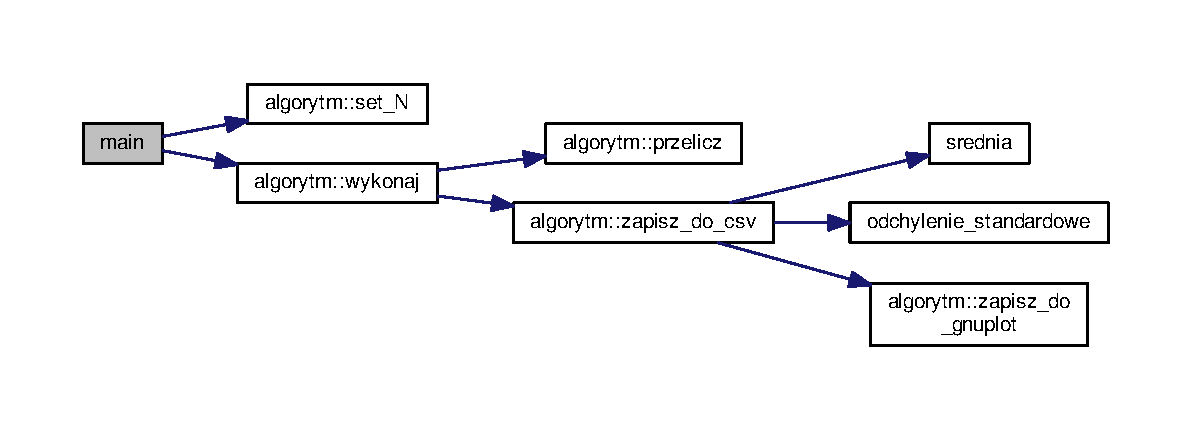
\includegraphics[width=350pt]{main_8cpp_ae66f6b31b5ad750f1fe042a706a4e3d4_cgraph}
\end{center}
\end{figure}



\hypertarget{operacje_8cpp}{\section{\-Dokumentacja pliku operacje.\-cpp}
\label{operacje_8cpp}\index{operacje.\-cpp@{operacje.\-cpp}}
}
{\ttfamily \#include \char`\"{}operacje.\-hh\char`\"{}}\*
\-Wykres zależności załączania dla operacje.\-cpp\-:\nopagebreak
\begin{figure}[H]
\begin{center}
\leavevmode
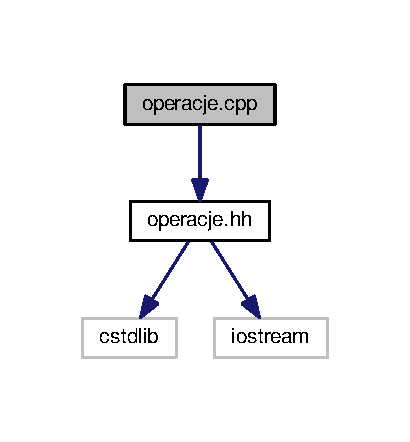
\includegraphics[width=196pt]{operacje_8cpp__incl}
\end{center}
\end{figure}

\hypertarget{operacje_8hh}{\section{\-Dokumentacja pliku operacje.\-hh}
\label{operacje_8hh}\index{operacje.\-hh@{operacje.\-hh}}
}
{\ttfamily \#include $<$cstdlib$>$}\*
{\ttfamily \#include $<$iostream$>$}\*
\-Wykres zależności załączania dla operacje.\-hh\-:
\nopagebreak
\begin{figure}[H]
\begin{center}
\leavevmode
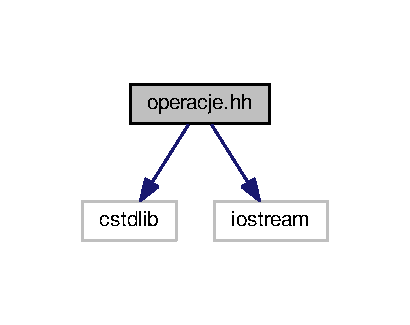
\includegraphics[width=196pt]{operacje_8hh__incl}
\end{center}
\end{figure}
\-Ten wykres pokazuje, które pliki bezpośrednio lub pośrednio załączają ten plik\-:
\nopagebreak
\begin{figure}[H]
\begin{center}
\leavevmode
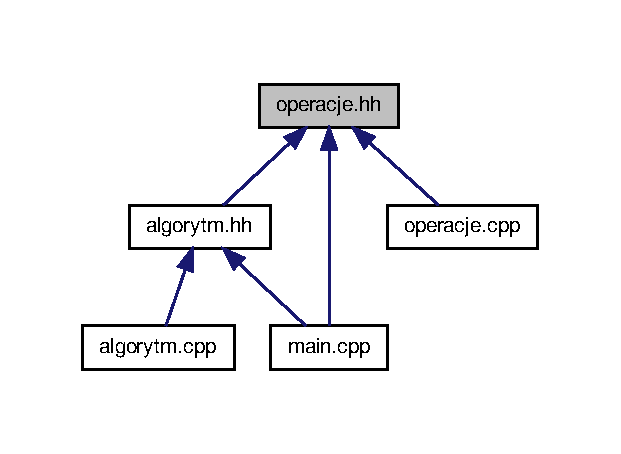
\includegraphics[width=298pt]{operacje_8hh__dep__incl}
\end{center}
\end{figure}
\subsection*{\-Komponenty}
\begin{DoxyCompactItemize}
\item 
class \hyperlink{classoperacje}{operacje}
\begin{DoxyCompactList}\small\item\em \-Klasa modeluje tablice z danymi i metody sluzace do operacji na niej. \end{DoxyCompactList}\end{DoxyCompactItemize}
\subsection*{\-Definicje}
\begin{DoxyCompactItemize}
\item 
\#define \hyperlink{operacje_8hh_aa50aa866c5823769bb02e986d29a0589}{\-R\-O\-Z\-M\-I\-A\-R}~9
\end{DoxyCompactItemize}


\subsection{\-Dokumentacja definicji}
\hypertarget{operacje_8hh_aa50aa866c5823769bb02e986d29a0589}{\index{operacje.\-hh@{operacje.\-hh}!\-R\-O\-Z\-M\-I\-A\-R@{\-R\-O\-Z\-M\-I\-A\-R}}
\index{\-R\-O\-Z\-M\-I\-A\-R@{\-R\-O\-Z\-M\-I\-A\-R}!operacje.hh@{operacje.\-hh}}
\subsubsection[{\-R\-O\-Z\-M\-I\-A\-R}]{\setlength{\rightskip}{0pt plus 5cm}\#define {\bf \-R\-O\-Z\-M\-I\-A\-R}~9}}\label{operacje_8hh_aa50aa866c5823769bb02e986d29a0589}


\-Definicja w linii 3 pliku operacje.\-hh.


\hypertarget{statystyki_8cpp}{\section{\-Dokumentacja pliku statystyki.\-cpp}
\label{statystyki_8cpp}\index{statystyki.\-cpp@{statystyki.\-cpp}}
}
{\ttfamily \#include \char`\"{}statystyki.\-hh\char`\"{}}\*
\-Wykres zależności załączania dla statystyki.\-cpp\-:\nopagebreak
\begin{figure}[H]
\begin{center}
\leavevmode
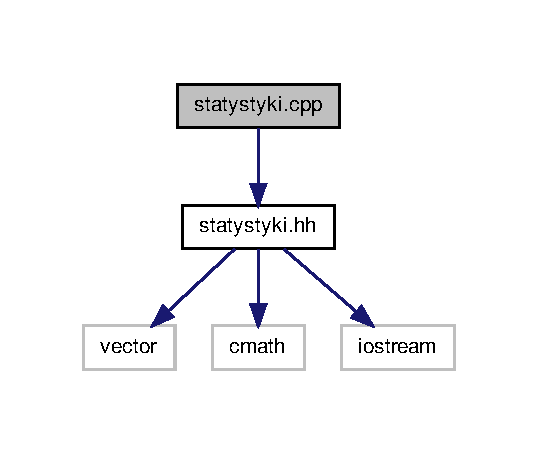
\includegraphics[width=258pt]{statystyki_8cpp__incl}
\end{center}
\end{figure}
\subsection*{\-Funkcje}
\begin{DoxyCompactItemize}
\item 
float \hyperlink{statystyki_8cpp_a978b972ebd4a834c47800d668ba8ecf2}{srednia} (float $\ast$tab, int rozmiar)
\begin{DoxyCompactList}\small\item\em funckja oblicza wartosc srednia \end{DoxyCompactList}\item 
float \hyperlink{statystyki_8cpp_a6648f32fbaacb03204231efea979cbf8}{odchylenie\-\_\-standardowe} (float \hyperlink{statystyki_8cpp_a978b972ebd4a834c47800d668ba8ecf2}{srednia}, float $\ast$tab, int rozmiar)
\begin{DoxyCompactList}\small\item\em funckja oblicza odchylenie standardowe \end{DoxyCompactList}\end{DoxyCompactItemize}


\subsection{\-Dokumentacja funkcji}
\hypertarget{statystyki_8cpp_a6648f32fbaacb03204231efea979cbf8}{\index{statystyki.\-cpp@{statystyki.\-cpp}!odchylenie\-\_\-standardowe@{odchylenie\-\_\-standardowe}}
\index{odchylenie\-\_\-standardowe@{odchylenie\-\_\-standardowe}!statystyki.cpp@{statystyki.\-cpp}}
\subsubsection[{odchylenie\-\_\-standardowe}]{\setlength{\rightskip}{0pt plus 5cm}float {\bf odchylenie\-\_\-standardowe} (
\begin{DoxyParamCaption}
\item[{float}]{srednia, }
\item[{float $\ast$}]{tab, }
\item[{int}]{rozmiar}
\end{DoxyParamCaption}
)}}\label{statystyki_8cpp_a6648f32fbaacb03204231efea979cbf8}


funckja oblicza odchylenie standardowe 


\begin{DoxyParams}{\-Parametry}
{\em tab} & -\/ kontener zawierajacy czasy wykonania algorytmu \\
\hline
{\em srednia} & -\/ wartosc srednia \\
\hline
{\em rozmiar} & -\/ rozmiar tablicy \\
\hline
\end{DoxyParams}
\begin{DoxyReturn}{\-Zwraca}
odchylenie standardowe 
\end{DoxyReturn}


\-Definicja w linii 16 pliku statystyki.\-cpp.



\-Oto graf wywoływań tej funkcji\-:\nopagebreak
\begin{figure}[H]
\begin{center}
\leavevmode
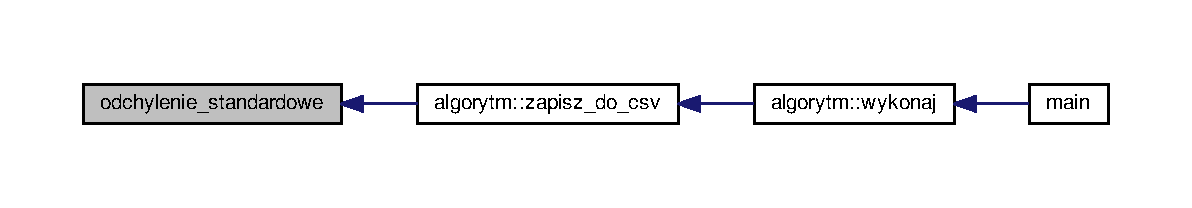
\includegraphics[width=350pt]{statystyki_8cpp_a6648f32fbaacb03204231efea979cbf8_icgraph}
\end{center}
\end{figure}


\hypertarget{statystyki_8cpp_a978b972ebd4a834c47800d668ba8ecf2}{\index{statystyki.\-cpp@{statystyki.\-cpp}!srednia@{srednia}}
\index{srednia@{srednia}!statystyki.cpp@{statystyki.\-cpp}}
\subsubsection[{srednia}]{\setlength{\rightskip}{0pt plus 5cm}float {\bf srednia} (
\begin{DoxyParamCaption}
\item[{float $\ast$}]{tab, }
\item[{int}]{rozmiar}
\end{DoxyParamCaption}
)}}\label{statystyki_8cpp_a978b972ebd4a834c47800d668ba8ecf2}


funckja oblicza wartosc srednia 


\begin{DoxyParams}{\-Parametry}
{\em tab} & -\/ kontener zawierajacy czasy wykonania algorytmu \\
\hline
{\em rozmiar} & -\/ rozmiar tablicy \\
\hline
\end{DoxyParams}
\begin{DoxyReturn}{\-Zwraca}
wartosc srednia 
\end{DoxyReturn}


\-Definicja w linii 3 pliku statystyki.\-cpp.



\-Oto graf wywoływań tej funkcji\-:\nopagebreak
\begin{figure}[H]
\begin{center}
\leavevmode
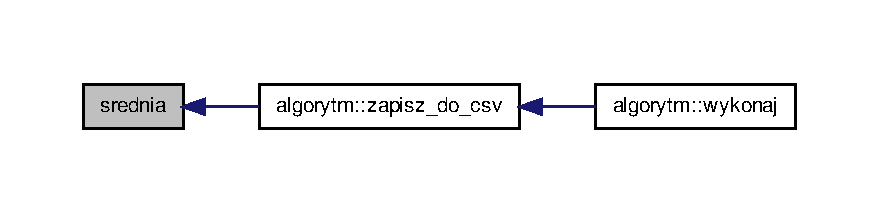
\includegraphics[width=350pt]{statystyki_8cpp_a978b972ebd4a834c47800d668ba8ecf2_icgraph}
\end{center}
\end{figure}



\hypertarget{statystyki_8hh}{\section{\-Dokumentacja pliku statystyki.\-hh}
\label{statystyki_8hh}\index{statystyki.\-hh@{statystyki.\-hh}}
}


plik zawiera dekalracje funkcji odpowiedzialnych za przeprowadznaie statystyk  


{\ttfamily \#include $<$vector$>$}\*
{\ttfamily \#include $<$cmath$>$}\*
{\ttfamily \#include $<$iostream$>$}\*
\-Wykres zależności załączania dla statystyki.\-hh\-:\nopagebreak
\begin{figure}[H]
\begin{center}
\leavevmode
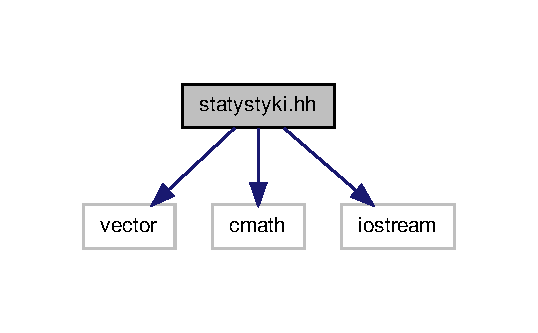
\includegraphics[width=258pt]{statystyki_8hh__incl}
\end{center}
\end{figure}
\-Ten wykres pokazuje, które pliki bezpośrednio lub pośrednio załączają ten plik\-:\nopagebreak
\begin{figure}[H]
\begin{center}
\leavevmode
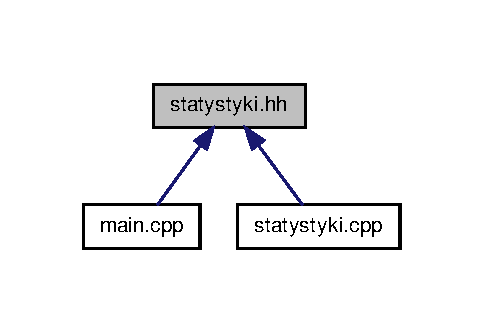
\includegraphics[width=322pt]{statystyki_8hh__dep__incl}
\end{center}
\end{figure}
\subsection*{\-Funkcje}
\begin{DoxyCompactItemize}
\item 
float \hyperlink{statystyki_8hh_a978b972ebd4a834c47800d668ba8ecf2}{srednia} (float $\ast$tab, int rozmiar)
\begin{DoxyCompactList}\small\item\em funckja oblicza wartosc srednia \end{DoxyCompactList}\item 
float \hyperlink{statystyki_8hh_a6648f32fbaacb03204231efea979cbf8}{odchylenie\-\_\-standardowe} (float \hyperlink{statystyki_8cpp_a978b972ebd4a834c47800d668ba8ecf2}{srednia}, float $\ast$tab, int rozmiar)
\begin{DoxyCompactList}\small\item\em funckja oblicza odchylenie standardowe \end{DoxyCompactList}\end{DoxyCompactItemize}


\subsection{\-Opis szczegółowy}
plik zawiera dekalracje funkcji odpowiedzialnych za przeprowadznaie statystyk 

\-Definicja w pliku \hyperlink{statystyki_8hh_source}{statystyki.\-hh}.



\subsection{\-Dokumentacja funkcji}
\hypertarget{statystyki_8hh_a6648f32fbaacb03204231efea979cbf8}{\index{statystyki.\-hh@{statystyki.\-hh}!odchylenie\-\_\-standardowe@{odchylenie\-\_\-standardowe}}
\index{odchylenie\-\_\-standardowe@{odchylenie\-\_\-standardowe}!statystyki.hh@{statystyki.\-hh}}
\subsubsection[{odchylenie\-\_\-standardowe}]{\setlength{\rightskip}{0pt plus 5cm}float {\bf odchylenie\-\_\-standardowe} (
\begin{DoxyParamCaption}
\item[{float}]{srednia, }
\item[{float $\ast$}]{tab, }
\item[{int}]{rozmiar}
\end{DoxyParamCaption}
)}}\label{statystyki_8hh_a6648f32fbaacb03204231efea979cbf8}


funckja oblicza odchylenie standardowe 


\begin{DoxyParams}{\-Parametry}
{\em tab} & -\/ kontener zawierajacy czasy wykonania algorytmu \\
\hline
{\em srednia} & -\/ wartosc srednia \\
\hline
{\em rozmiar} & -\/ rozmiar tablicy \\
\hline
\end{DoxyParams}
\begin{DoxyReturn}{\-Zwraca}
odchylenie standardowe 
\end{DoxyReturn}


\-Definicja w linii 16 pliku statystyki.\-cpp.



\-Oto graf wywoływań tej funkcji\-:\nopagebreak
\begin{figure}[H]
\begin{center}
\leavevmode
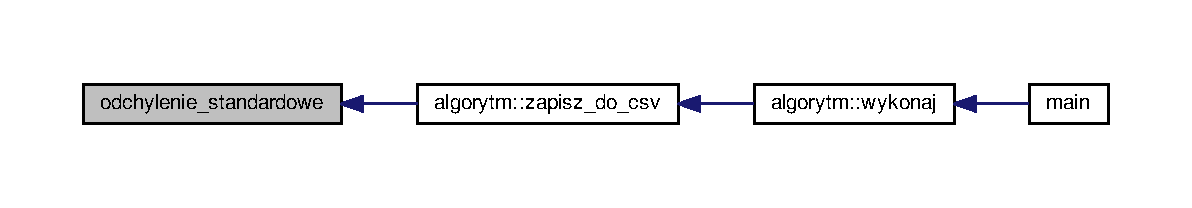
\includegraphics[width=350pt]{statystyki_8hh_a6648f32fbaacb03204231efea979cbf8_icgraph}
\end{center}
\end{figure}


\hypertarget{statystyki_8hh_a978b972ebd4a834c47800d668ba8ecf2}{\index{statystyki.\-hh@{statystyki.\-hh}!srednia@{srednia}}
\index{srednia@{srednia}!statystyki.hh@{statystyki.\-hh}}
\subsubsection[{srednia}]{\setlength{\rightskip}{0pt plus 5cm}float {\bf srednia} (
\begin{DoxyParamCaption}
\item[{float $\ast$}]{tab, }
\item[{int}]{rozmiar}
\end{DoxyParamCaption}
)}}\label{statystyki_8hh_a978b972ebd4a834c47800d668ba8ecf2}


funckja oblicza wartosc srednia 


\begin{DoxyParams}{\-Parametry}
{\em tab} & -\/ kontener zawierajacy czasy wykonania algorytmu \\
\hline
{\em rozmiar} & -\/ rozmiar tablicy \\
\hline
\end{DoxyParams}
\begin{DoxyReturn}{\-Zwraca}
wartosc srednia 
\end{DoxyReturn}


\-Definicja w linii 3 pliku statystyki.\-cpp.



\-Oto graf wywoływań tej funkcji\-:\nopagebreak
\begin{figure}[H]
\begin{center}
\leavevmode
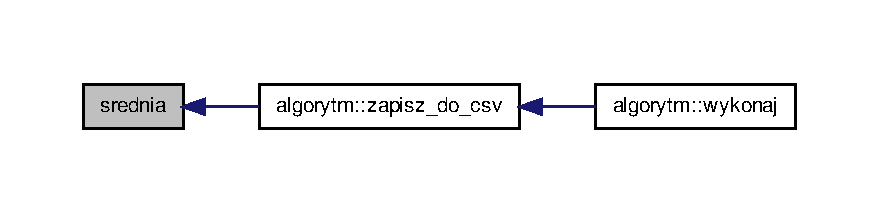
\includegraphics[width=350pt]{statystyki_8hh_a978b972ebd4a834c47800d668ba8ecf2_icgraph}
\end{center}
\end{figure}



\hypertarget{strona_8dox}{\section{\-Dokumentacja pliku strona.\-dox}
\label{strona_8dox}\index{strona.\-dox@{strona.\-dox}}
}

\printindex
\end{document}
